% generated by gen_div_fig.py -- do not edit by hand
\documentclass[10pt]{standalone}
\usepackage{helvet}
\renewcommand{\familydefault}{\sfdefault}
\usepackage{amsmath,amssymb}
\usepackage{tikz}
\usetikzlibrary{arrows.meta,patterns,decorations.pathreplacing}
\definecolor{dA}{HTML}{481D6F}
\definecolor{dB}{HTML}{2E6F8E}
\definecolor{dC}{HTML}{2CB17E}
\definecolor{dD}{HTML}{CAE11F}
\definecolor{cpop}{HTML}{C55A11}
\newcommand{\fs}{\fontsize{6.4}{7.4}\selectfont}
\newcommand{\fss}{\fontsize{5.8}{6.6}\selectfont}
\begin{document}
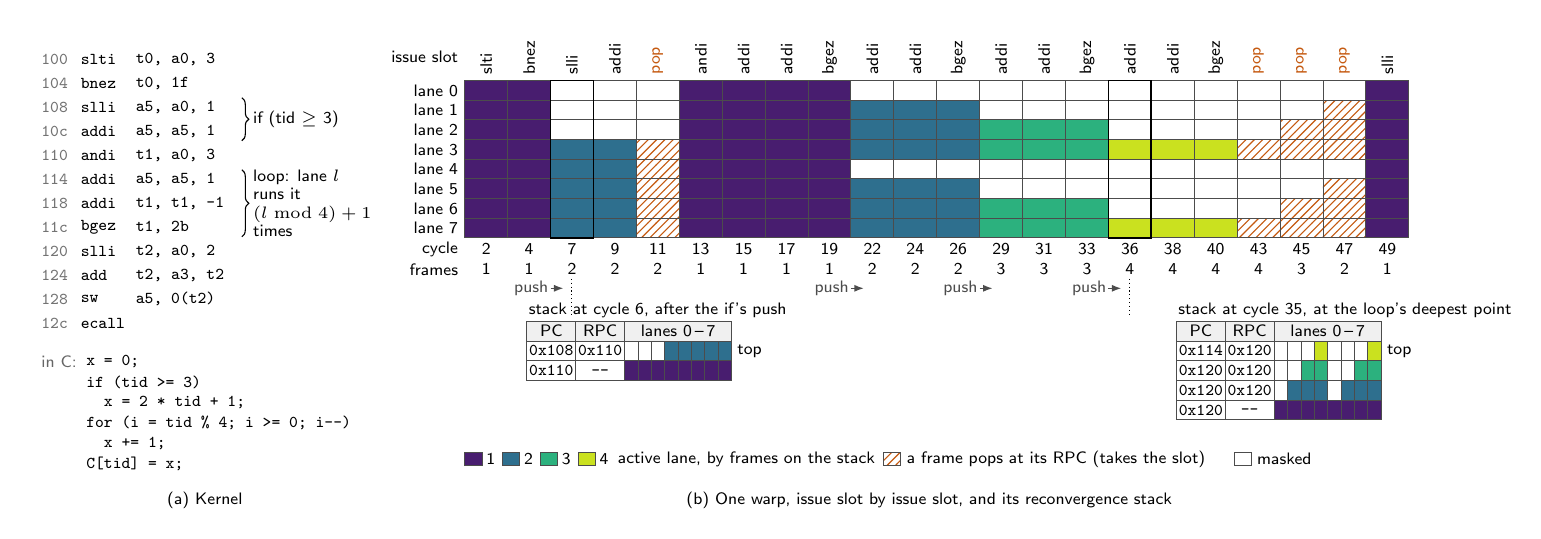
\begin{tikzpicture}[x=1cm, y=1cm,
  tbl/.style={draw=black!70, line width=0.3pt},
  lbl/.style={font=\fs, inner sep=0.5pt},
  note/.style={font=\fss, inner sep=0.5pt, align=left},
  code/.style={font=\fss\ttfamily, inner sep=0.5pt, anchor=west},
  panel/.style={draw=none, fill=none},
  subcap/.style={font=\fs, inner sep=1pt},
  arr/.style={-{Latex[length=1.2mm, width=0.9mm]}, line width=0.5pt}]

\draw[panel] (-0.100,-0.050) rectangle (4.400,5.650);
\node[code, text=black!55] at (0.05,5.250) {100};
\node[code] at (0.55,5.250) {slti};
\node[code] at (1.25,5.250) {t0, a0, 3};
\node[code, text=black!55] at (0.05,4.945) {104};
\node[code] at (0.55,4.945) {bnez};
\node[code] at (1.25,4.945) {t0, 1f};
\node[code, text=black!55] at (0.05,4.640) {108};
\node[code] at (0.55,4.640) {slli};
\node[code] at (1.25,4.640) {a5, a0, 1};
\node[code, text=black!55] at (0.05,4.335) {10c};
\node[code] at (0.55,4.335) {addi};
\node[code] at (1.25,4.335) {a5, a5, 1};
\node[code, text=black!55] at (0.05,4.030) {110};
\node[code] at (0.55,4.030) {andi};
\node[code] at (1.25,4.030) {t1, a0, 3};
\node[code, text=black!55] at (0.05,3.725) {114};
\node[code] at (0.55,3.725) {addi};
\node[code] at (1.25,3.725) {a5, a5, 1};
\node[code, text=black!55] at (0.05,3.420) {118};
\node[code] at (0.55,3.420) {addi};
\node[code] at (1.25,3.420) {t1, t1, -1};
\node[code, text=black!55] at (0.05,3.115) {11c};
\node[code] at (0.55,3.115) {bgez};
\node[code] at (1.25,3.115) {t1, 2b};
\node[code, text=black!55] at (0.05,2.810) {120};
\node[code] at (0.55,2.810) {slli};
\node[code] at (1.25,2.810) {t2, a0, 2};
\node[code, text=black!55] at (0.05,2.505) {124};
\node[code] at (0.55,2.505) {add};
\node[code] at (1.25,2.505) {t2, a3, t2};
\node[code, text=black!55] at (0.05,2.200) {128};
\node[code] at (0.55,2.200) {sw};
\node[code] at (1.25,2.200) {a5, 0(t2)};
\node[code, text=black!55] at (0.05,1.895) {12c};
\node[code] at (0.55,1.895) {ecall};
\node[code] at (1.25,1.895) {};
\draw[decorate, decoration={brace, amplitude=2.5pt}, line width=0.4pt] (2.62,4.760) -- (2.62,4.215);
\node[note, anchor=west] at (2.74,4.487) {if (tid $\geq$ 3)};
\draw[decorate, decoration={brace, amplitude=2.5pt}, line width=0.4pt] (2.62,3.845) -- (2.62,2.995);
\node[note, anchor=west] at (2.74,3.420) {loop: lane $l$\\runs it\\$(l \bmod 4)+1$\\times};
\node[note, anchor=west, text=black!60] at (0.05,1.410) {in C:};
\node[code] at (0.62,1.410) {x = 0;};
\node[code] at (0.62,1.150) {if (tid >= 3)};
\node[code] at (0.62,0.890) {\ \ x = 2 * tid + 1;};
\node[code] at (0.62,0.630) {for (i = tid \% 4; i >= 0; i--)};
\node[code] at (0.62,0.370) {\ \ x += 1;};
\node[code] at (0.62,0.110) {C[tid] = x;};
\node[subcap] at (2.150,-0.350) {(a) Kernel};
\draw[panel] (4.550,-0.050) rectangle (18.150,5.650);
\node[lbl, anchor=east] at (5.390,4.855) {lane 0};
\node[lbl, anchor=east] at (5.390,4.605) {lane 1};
\node[lbl, anchor=east] at (5.390,4.355) {lane 2};
\node[lbl, anchor=east] at (5.390,4.105) {lane 3};
\node[lbl, anchor=east] at (5.390,3.855) {lane 4};
\node[lbl, anchor=east] at (5.390,3.605) {lane 5};
\node[lbl, anchor=east] at (5.390,3.355) {lane 6};
\node[lbl, anchor=east] at (5.390,3.105) {lane 7};
\draw[tbl, fill=dA] (5.450,4.730) rectangle (5.995,4.980);
\draw[tbl, fill=dA] (5.450,4.480) rectangle (5.995,4.730);
\draw[tbl, fill=dA] (5.450,4.230) rectangle (5.995,4.480);
\draw[tbl, fill=dA] (5.450,3.980) rectangle (5.995,4.230);
\draw[tbl, fill=dA] (5.450,3.730) rectangle (5.995,3.980);
\draw[tbl, fill=dA] (5.450,3.480) rectangle (5.995,3.730);
\draw[tbl, fill=dA] (5.450,3.230) rectangle (5.995,3.480);
\draw[tbl, fill=dA] (5.450,2.980) rectangle (5.995,3.230);
\node[lbl, text=black, rotate=90, anchor=west] at (5.723,5.030) {slti};
\node[note] at (5.723,2.840) {2};
\node[note] at (5.723,2.580) {1};
\draw[tbl, fill=dA] (5.995,4.730) rectangle (6.540,4.980);
\draw[tbl, fill=dA] (5.995,4.480) rectangle (6.540,4.730);
\draw[tbl, fill=dA] (5.995,4.230) rectangle (6.540,4.480);
\draw[tbl, fill=dA] (5.995,3.980) rectangle (6.540,4.230);
\draw[tbl, fill=dA] (5.995,3.730) rectangle (6.540,3.980);
\draw[tbl, fill=dA] (5.995,3.480) rectangle (6.540,3.730);
\draw[tbl, fill=dA] (5.995,3.230) rectangle (6.540,3.480);
\draw[tbl, fill=dA] (5.995,2.980) rectangle (6.540,3.230);
\node[lbl, text=black, rotate=90, anchor=west] at (6.268,5.030) {bnez};
\node[note] at (6.268,2.840) {4};
\node[note] at (6.268,2.580) {1};
\draw[arr, draw=black!70] (6.540,2.340) -- (6.704,2.340);
\node[note, text=black!70] at (6.295,2.340) {push};
\draw[tbl, fill=white] (6.540,4.730) rectangle (7.085,4.980);
\draw[tbl, fill=white] (6.540,4.480) rectangle (7.085,4.730);
\draw[tbl, fill=white] (6.540,4.230) rectangle (7.085,4.480);
\draw[tbl, fill=dB] (6.540,3.980) rectangle (7.085,4.230);
\draw[tbl, fill=dB] (6.540,3.730) rectangle (7.085,3.980);
\draw[tbl, fill=dB] (6.540,3.480) rectangle (7.085,3.730);
\draw[tbl, fill=dB] (6.540,3.230) rectangle (7.085,3.480);
\draw[tbl, fill=dB] (6.540,2.980) rectangle (7.085,3.230);
\node[lbl, text=black, rotate=90, anchor=west] at (6.812,5.030) {slli};
\node[note] at (6.812,2.840) {7};
\node[note] at (6.812,2.580) {2};
\draw[tbl, fill=white] (7.085,4.730) rectangle (7.630,4.980);
\draw[tbl, fill=white] (7.085,4.480) rectangle (7.630,4.730);
\draw[tbl, fill=white] (7.085,4.230) rectangle (7.630,4.480);
\draw[tbl, fill=dB] (7.085,3.980) rectangle (7.630,4.230);
\draw[tbl, fill=dB] (7.085,3.730) rectangle (7.630,3.980);
\draw[tbl, fill=dB] (7.085,3.480) rectangle (7.630,3.730);
\draw[tbl, fill=dB] (7.085,3.230) rectangle (7.630,3.480);
\draw[tbl, fill=dB] (7.085,2.980) rectangle (7.630,3.230);
\node[lbl, text=black, rotate=90, anchor=west] at (7.358,5.030) {addi};
\node[note] at (7.358,2.840) {9};
\node[note] at (7.358,2.580) {2};
\draw[tbl, fill=white] (7.630,4.730) rectangle (8.175,4.980);
\draw[tbl, fill=white] (7.630,4.480) rectangle (8.175,4.730);
\draw[tbl, fill=white] (7.630,4.230) rectangle (8.175,4.480);
\draw[tbl, pattern=north east lines, pattern color=cpop] (7.630,3.980) rectangle (8.175,4.230);
\draw[tbl, pattern=north east lines, pattern color=cpop] (7.630,3.730) rectangle (8.175,3.980);
\draw[tbl, pattern=north east lines, pattern color=cpop] (7.630,3.480) rectangle (8.175,3.730);
\draw[tbl, pattern=north east lines, pattern color=cpop] (7.630,3.230) rectangle (8.175,3.480);
\draw[tbl, pattern=north east lines, pattern color=cpop] (7.630,2.980) rectangle (8.175,3.230);
\node[lbl, text=cpop, rotate=90, anchor=west] at (7.903,5.030) {pop};
\node[note] at (7.903,2.840) {11};
\node[note] at (7.903,2.580) {2};
\draw[tbl, fill=dA] (8.175,4.730) rectangle (8.720,4.980);
\draw[tbl, fill=dA] (8.175,4.480) rectangle (8.720,4.730);
\draw[tbl, fill=dA] (8.175,4.230) rectangle (8.720,4.480);
\draw[tbl, fill=dA] (8.175,3.980) rectangle (8.720,4.230);
\draw[tbl, fill=dA] (8.175,3.730) rectangle (8.720,3.980);
\draw[tbl, fill=dA] (8.175,3.480) rectangle (8.720,3.730);
\draw[tbl, fill=dA] (8.175,3.230) rectangle (8.720,3.480);
\draw[tbl, fill=dA] (8.175,2.980) rectangle (8.720,3.230);
\node[lbl, text=black, rotate=90, anchor=west] at (8.448,5.030) {andi};
\node[note] at (8.448,2.840) {13};
\node[note] at (8.448,2.580) {1};
\draw[tbl, fill=dA] (8.720,4.730) rectangle (9.265,4.980);
\draw[tbl, fill=dA] (8.720,4.480) rectangle (9.265,4.730);
\draw[tbl, fill=dA] (8.720,4.230) rectangle (9.265,4.480);
\draw[tbl, fill=dA] (8.720,3.980) rectangle (9.265,4.230);
\draw[tbl, fill=dA] (8.720,3.730) rectangle (9.265,3.980);
\draw[tbl, fill=dA] (8.720,3.480) rectangle (9.265,3.730);
\draw[tbl, fill=dA] (8.720,3.230) rectangle (9.265,3.480);
\draw[tbl, fill=dA] (8.720,2.980) rectangle (9.265,3.230);
\node[lbl, text=black, rotate=90, anchor=west] at (8.993,5.030) {addi};
\node[note] at (8.993,2.840) {15};
\node[note] at (8.993,2.580) {1};
\draw[tbl, fill=dA] (9.265,4.730) rectangle (9.810,4.980);
\draw[tbl, fill=dA] (9.265,4.480) rectangle (9.810,4.730);
\draw[tbl, fill=dA] (9.265,4.230) rectangle (9.810,4.480);
\draw[tbl, fill=dA] (9.265,3.980) rectangle (9.810,4.230);
\draw[tbl, fill=dA] (9.265,3.730) rectangle (9.810,3.980);
\draw[tbl, fill=dA] (9.265,3.480) rectangle (9.810,3.730);
\draw[tbl, fill=dA] (9.265,3.230) rectangle (9.810,3.480);
\draw[tbl, fill=dA] (9.265,2.980) rectangle (9.810,3.230);
\node[lbl, text=black, rotate=90, anchor=west] at (9.538,5.030) {addi};
\node[note] at (9.538,2.840) {17};
\node[note] at (9.538,2.580) {1};
\draw[tbl, fill=dA] (9.810,4.730) rectangle (10.355,4.980);
\draw[tbl, fill=dA] (9.810,4.480) rectangle (10.355,4.730);
\draw[tbl, fill=dA] (9.810,4.230) rectangle (10.355,4.480);
\draw[tbl, fill=dA] (9.810,3.980) rectangle (10.355,4.230);
\draw[tbl, fill=dA] (9.810,3.730) rectangle (10.355,3.980);
\draw[tbl, fill=dA] (9.810,3.480) rectangle (10.355,3.730);
\draw[tbl, fill=dA] (9.810,3.230) rectangle (10.355,3.480);
\draw[tbl, fill=dA] (9.810,2.980) rectangle (10.355,3.230);
\node[lbl, text=black, rotate=90, anchor=west] at (10.083,5.030) {bgez};
\node[note] at (10.083,2.840) {19};
\node[note] at (10.083,2.580) {1};
\draw[arr, draw=black!70] (10.355,2.340) -- (10.519,2.340);
\node[note, text=black!70] at (10.110,2.340) {push};
\draw[tbl, fill=white] (10.355,4.730) rectangle (10.900,4.980);
\draw[tbl, fill=dB] (10.355,4.480) rectangle (10.900,4.730);
\draw[tbl, fill=dB] (10.355,4.230) rectangle (10.900,4.480);
\draw[tbl, fill=dB] (10.355,3.980) rectangle (10.900,4.230);
\draw[tbl, fill=white] (10.355,3.730) rectangle (10.900,3.980);
\draw[tbl, fill=dB] (10.355,3.480) rectangle (10.900,3.730);
\draw[tbl, fill=dB] (10.355,3.230) rectangle (10.900,3.480);
\draw[tbl, fill=dB] (10.355,2.980) rectangle (10.900,3.230);
\node[lbl, text=black, rotate=90, anchor=west] at (10.628,5.030) {addi};
\node[note] at (10.628,2.840) {22};
\node[note] at (10.628,2.580) {2};
\draw[tbl, fill=white] (10.900,4.730) rectangle (11.445,4.980);
\draw[tbl, fill=dB] (10.900,4.480) rectangle (11.445,4.730);
\draw[tbl, fill=dB] (10.900,4.230) rectangle (11.445,4.480);
\draw[tbl, fill=dB] (10.900,3.980) rectangle (11.445,4.230);
\draw[tbl, fill=white] (10.900,3.730) rectangle (11.445,3.980);
\draw[tbl, fill=dB] (10.900,3.480) rectangle (11.445,3.730);
\draw[tbl, fill=dB] (10.900,3.230) rectangle (11.445,3.480);
\draw[tbl, fill=dB] (10.900,2.980) rectangle (11.445,3.230);
\node[lbl, text=black, rotate=90, anchor=west] at (11.173,5.030) {addi};
\node[note] at (11.173,2.840) {24};
\node[note] at (11.173,2.580) {2};
\draw[tbl, fill=white] (11.445,4.730) rectangle (11.990,4.980);
\draw[tbl, fill=dB] (11.445,4.480) rectangle (11.990,4.730);
\draw[tbl, fill=dB] (11.445,4.230) rectangle (11.990,4.480);
\draw[tbl, fill=dB] (11.445,3.980) rectangle (11.990,4.230);
\draw[tbl, fill=white] (11.445,3.730) rectangle (11.990,3.980);
\draw[tbl, fill=dB] (11.445,3.480) rectangle (11.990,3.730);
\draw[tbl, fill=dB] (11.445,3.230) rectangle (11.990,3.480);
\draw[tbl, fill=dB] (11.445,2.980) rectangle (11.990,3.230);
\node[lbl, text=black, rotate=90, anchor=west] at (11.718,5.030) {bgez};
\node[note] at (11.718,2.840) {26};
\node[note] at (11.718,2.580) {2};
\draw[arr, draw=black!70] (11.990,2.340) -- (12.154,2.340);
\node[note, text=black!70] at (11.745,2.340) {push};
\draw[tbl, fill=white] (11.990,4.730) rectangle (12.535,4.980);
\draw[tbl, fill=white] (11.990,4.480) rectangle (12.535,4.730);
\draw[tbl, fill=dC] (11.990,4.230) rectangle (12.535,4.480);
\draw[tbl, fill=dC] (11.990,3.980) rectangle (12.535,4.230);
\draw[tbl, fill=white] (11.990,3.730) rectangle (12.535,3.980);
\draw[tbl, fill=white] (11.990,3.480) rectangle (12.535,3.730);
\draw[tbl, fill=dC] (11.990,3.230) rectangle (12.535,3.480);
\draw[tbl, fill=dC] (11.990,2.980) rectangle (12.535,3.230);
\node[lbl, text=black, rotate=90, anchor=west] at (12.263,5.030) {addi};
\node[note] at (12.263,2.840) {29};
\node[note] at (12.263,2.580) {3};
\draw[tbl, fill=white] (12.535,4.730) rectangle (13.080,4.980);
\draw[tbl, fill=white] (12.535,4.480) rectangle (13.080,4.730);
\draw[tbl, fill=dC] (12.535,4.230) rectangle (13.080,4.480);
\draw[tbl, fill=dC] (12.535,3.980) rectangle (13.080,4.230);
\draw[tbl, fill=white] (12.535,3.730) rectangle (13.080,3.980);
\draw[tbl, fill=white] (12.535,3.480) rectangle (13.080,3.730);
\draw[tbl, fill=dC] (12.535,3.230) rectangle (13.080,3.480);
\draw[tbl, fill=dC] (12.535,2.980) rectangle (13.080,3.230);
\node[lbl, text=black, rotate=90, anchor=west] at (12.808,5.030) {addi};
\node[note] at (12.808,2.840) {31};
\node[note] at (12.808,2.580) {3};
\draw[tbl, fill=white] (13.080,4.730) rectangle (13.625,4.980);
\draw[tbl, fill=white] (13.080,4.480) rectangle (13.625,4.730);
\draw[tbl, fill=dC] (13.080,4.230) rectangle (13.625,4.480);
\draw[tbl, fill=dC] (13.080,3.980) rectangle (13.625,4.230);
\draw[tbl, fill=white] (13.080,3.730) rectangle (13.625,3.980);
\draw[tbl, fill=white] (13.080,3.480) rectangle (13.625,3.730);
\draw[tbl, fill=dC] (13.080,3.230) rectangle (13.625,3.480);
\draw[tbl, fill=dC] (13.080,2.980) rectangle (13.625,3.230);
\node[lbl, text=black, rotate=90, anchor=west] at (13.353,5.030) {bgez};
\node[note] at (13.353,2.840) {33};
\node[note] at (13.353,2.580) {3};
\draw[arr, draw=black!70] (13.625,2.340) -- (13.789,2.340);
\node[note, text=black!70] at (13.380,2.340) {push};
\draw[tbl, fill=white] (13.625,4.730) rectangle (14.170,4.980);
\draw[tbl, fill=white] (13.625,4.480) rectangle (14.170,4.730);
\draw[tbl, fill=white] (13.625,4.230) rectangle (14.170,4.480);
\draw[tbl, fill=dD] (13.625,3.980) rectangle (14.170,4.230);
\draw[tbl, fill=white] (13.625,3.730) rectangle (14.170,3.980);
\draw[tbl, fill=white] (13.625,3.480) rectangle (14.170,3.730);
\draw[tbl, fill=white] (13.625,3.230) rectangle (14.170,3.480);
\draw[tbl, fill=dD] (13.625,2.980) rectangle (14.170,3.230);
\node[lbl, text=black, rotate=90, anchor=west] at (13.898,5.030) {addi};
\node[note] at (13.898,2.840) {36};
\node[note] at (13.898,2.580) {4};
\draw[tbl, fill=white] (14.170,4.730) rectangle (14.715,4.980);
\draw[tbl, fill=white] (14.170,4.480) rectangle (14.715,4.730);
\draw[tbl, fill=white] (14.170,4.230) rectangle (14.715,4.480);
\draw[tbl, fill=dD] (14.170,3.980) rectangle (14.715,4.230);
\draw[tbl, fill=white] (14.170,3.730) rectangle (14.715,3.980);
\draw[tbl, fill=white] (14.170,3.480) rectangle (14.715,3.730);
\draw[tbl, fill=white] (14.170,3.230) rectangle (14.715,3.480);
\draw[tbl, fill=dD] (14.170,2.980) rectangle (14.715,3.230);
\node[lbl, text=black, rotate=90, anchor=west] at (14.443,5.030) {addi};
\node[note] at (14.443,2.840) {38};
\node[note] at (14.443,2.580) {4};
\draw[tbl, fill=white] (14.715,4.730) rectangle (15.260,4.980);
\draw[tbl, fill=white] (14.715,4.480) rectangle (15.260,4.730);
\draw[tbl, fill=white] (14.715,4.230) rectangle (15.260,4.480);
\draw[tbl, fill=dD] (14.715,3.980) rectangle (15.260,4.230);
\draw[tbl, fill=white] (14.715,3.730) rectangle (15.260,3.980);
\draw[tbl, fill=white] (14.715,3.480) rectangle (15.260,3.730);
\draw[tbl, fill=white] (14.715,3.230) rectangle (15.260,3.480);
\draw[tbl, fill=dD] (14.715,2.980) rectangle (15.260,3.230);
\node[lbl, text=black, rotate=90, anchor=west] at (14.988,5.030) {bgez};
\node[note] at (14.988,2.840) {40};
\node[note] at (14.988,2.580) {4};
\draw[tbl, fill=white] (15.260,4.730) rectangle (15.805,4.980);
\draw[tbl, fill=white] (15.260,4.480) rectangle (15.805,4.730);
\draw[tbl, fill=white] (15.260,4.230) rectangle (15.805,4.480);
\draw[tbl, pattern=north east lines, pattern color=cpop] (15.260,3.980) rectangle (15.805,4.230);
\draw[tbl, fill=white] (15.260,3.730) rectangle (15.805,3.980);
\draw[tbl, fill=white] (15.260,3.480) rectangle (15.805,3.730);
\draw[tbl, fill=white] (15.260,3.230) rectangle (15.805,3.480);
\draw[tbl, pattern=north east lines, pattern color=cpop] (15.260,2.980) rectangle (15.805,3.230);
\node[lbl, text=cpop, rotate=90, anchor=west] at (15.533,5.030) {pop};
\node[note] at (15.533,2.840) {43};
\node[note] at (15.533,2.580) {4};
\draw[tbl, fill=white] (15.805,4.730) rectangle (16.350,4.980);
\draw[tbl, fill=white] (15.805,4.480) rectangle (16.350,4.730);
\draw[tbl, pattern=north east lines, pattern color=cpop] (15.805,4.230) rectangle (16.350,4.480);
\draw[tbl, pattern=north east lines, pattern color=cpop] (15.805,3.980) rectangle (16.350,4.230);
\draw[tbl, fill=white] (15.805,3.730) rectangle (16.350,3.980);
\draw[tbl, fill=white] (15.805,3.480) rectangle (16.350,3.730);
\draw[tbl, pattern=north east lines, pattern color=cpop] (15.805,3.230) rectangle (16.350,3.480);
\draw[tbl, pattern=north east lines, pattern color=cpop] (15.805,2.980) rectangle (16.350,3.230);
\node[lbl, text=cpop, rotate=90, anchor=west] at (16.078,5.030) {pop};
\node[note] at (16.078,2.840) {45};
\node[note] at (16.078,2.580) {3};
\draw[tbl, fill=white] (16.350,4.730) rectangle (16.895,4.980);
\draw[tbl, pattern=north east lines, pattern color=cpop] (16.350,4.480) rectangle (16.895,4.730);
\draw[tbl, pattern=north east lines, pattern color=cpop] (16.350,4.230) rectangle (16.895,4.480);
\draw[tbl, pattern=north east lines, pattern color=cpop] (16.350,3.980) rectangle (16.895,4.230);
\draw[tbl, fill=white] (16.350,3.730) rectangle (16.895,3.980);
\draw[tbl, pattern=north east lines, pattern color=cpop] (16.350,3.480) rectangle (16.895,3.730);
\draw[tbl, pattern=north east lines, pattern color=cpop] (16.350,3.230) rectangle (16.895,3.480);
\draw[tbl, pattern=north east lines, pattern color=cpop] (16.350,2.980) rectangle (16.895,3.230);
\node[lbl, text=cpop, rotate=90, anchor=west] at (16.623,5.030) {pop};
\node[note] at (16.623,2.840) {47};
\node[note] at (16.623,2.580) {2};
\draw[tbl, fill=dA] (16.895,4.730) rectangle (17.440,4.980);
\draw[tbl, fill=dA] (16.895,4.480) rectangle (17.440,4.730);
\draw[tbl, fill=dA] (16.895,4.230) rectangle (17.440,4.480);
\draw[tbl, fill=dA] (16.895,3.980) rectangle (17.440,4.230);
\draw[tbl, fill=dA] (16.895,3.730) rectangle (17.440,3.980);
\draw[tbl, fill=dA] (16.895,3.480) rectangle (17.440,3.730);
\draw[tbl, fill=dA] (16.895,3.230) rectangle (17.440,3.480);
\draw[tbl, fill=dA] (16.895,2.980) rectangle (17.440,3.230);
\node[lbl, text=black, rotate=90, anchor=west] at (17.168,5.030) {slli};
\node[note] at (17.168,2.840) {49};
\node[note] at (17.168,2.580) {1};
\node[note, anchor=east] at (5.390,2.840) {cycle};
\node[note, anchor=east] at (5.390,2.580) {frames};
\node[lbl, anchor=east] at (5.390,5.280) {issue slot};
\draw[tbl, fill=dA] (5.450,0.090) rectangle (5.670,0.250);
\node[note, anchor=west] at (5.700,0.170) {1};
\draw[tbl, fill=dB] (5.930,0.090) rectangle (6.150,0.250);
\node[note, anchor=west] at (6.180,0.170) {2};
\draw[tbl, fill=dC] (6.410,0.090) rectangle (6.630,0.250);
\node[note, anchor=west] at (6.660,0.170) {3};
\draw[tbl, fill=dD] (6.890,0.090) rectangle (7.110,0.250);
\node[note, anchor=west] at (7.140,0.170) {4};
\node[note, anchor=west] at (7.370,0.170) {active lane, by frames on the stack};
\draw[tbl, pattern=north east lines, pattern color=cpop] (10.770,0.090) rectangle (10.990,0.250);
\node[note, anchor=west] at (11.040,0.170) {a frame pops at its RPC (takes the slot)};
\draw[tbl, fill=white] (15.220,0.090) rectangle (15.440,0.250);
\node[note, anchor=west] at (15.490,0.170) {masked};
\draw[tbl, draw=black, line width=0.6pt] (6.540,2.980) rectangle (7.085,4.980);
\draw[line width=0.4pt, densely dotted] (6.812,2.460) -- (6.812,1.980);
\node[note, anchor=south west] at (6.240,1.940) {stack at cycle 6, after the if's push};
\draw[tbl, fill=black!6] (6.240,1.670) rectangle (6.860,1.920);
\node[note] at (6.550,1.795) {PC};
\draw[tbl, fill=black!6] (6.860,1.670) rectangle (7.480,1.920);
\node[note] at (7.170,1.795) {RPC};
\draw[tbl, fill=black!6] (7.480,1.670) rectangle (8.840,1.920);
\node[note] at (8.160,1.795) {lanes 0\,--\,7};
\draw[tbl] (6.240,1.420) rectangle (6.860,1.670);
\node[note, font=\fss\ttfamily] at (6.550,1.545) {0x108};
\draw[tbl] (6.860,1.420) rectangle (7.480,1.670);
\node[note, font=\fss\ttfamily] at (7.170,1.545) {0x110};
\draw[tbl, fill=white] (7.480,1.420) rectangle (7.650,1.670);
\draw[tbl, fill=white] (7.650,1.420) rectangle (7.820,1.670);
\draw[tbl, fill=white] (7.820,1.420) rectangle (7.990,1.670);
\draw[tbl, fill=dB] (7.990,1.420) rectangle (8.160,1.670);
\draw[tbl, fill=dB] (8.160,1.420) rectangle (8.330,1.670);
\draw[tbl, fill=dB] (8.330,1.420) rectangle (8.500,1.670);
\draw[tbl, fill=dB] (8.500,1.420) rectangle (8.670,1.670);
\draw[tbl, fill=dB] (8.670,1.420) rectangle (8.840,1.670);
\node[note, anchor=west] at (8.890,1.545) {top};
\draw[tbl] (6.240,1.170) rectangle (6.860,1.420);
\node[note, font=\fss\ttfamily] at (6.550,1.295) {0x110};
\draw[tbl] (6.860,1.170) rectangle (7.480,1.420);
\node[note, font=\fss\ttfamily] at (7.170,1.295) {--};
\draw[tbl, fill=dA] (7.480,1.170) rectangle (7.650,1.420);
\draw[tbl, fill=dA] (7.650,1.170) rectangle (7.820,1.420);
\draw[tbl, fill=dA] (7.820,1.170) rectangle (7.990,1.420);
\draw[tbl, fill=dA] (7.990,1.170) rectangle (8.160,1.420);
\draw[tbl, fill=dA] (8.160,1.170) rectangle (8.330,1.420);
\draw[tbl, fill=dA] (8.330,1.170) rectangle (8.500,1.420);
\draw[tbl, fill=dA] (8.500,1.170) rectangle (8.670,1.420);
\draw[tbl, fill=dA] (8.670,1.170) rectangle (8.840,1.420);
\node[note, anchor=west] at (8.890,1.295) {};
\draw[tbl, draw=black, line width=0.6pt] (13.625,2.980) rectangle (14.170,4.980);
\draw[line width=0.4pt, densely dotted] (13.898,2.460) -- (13.898,1.980);
\node[note, anchor=south west] at (14.490,1.940) {stack at cycle 35, at the loop's deepest point};
\draw[tbl, fill=black!6] (14.490,1.670) rectangle (15.110,1.920);
\node[note] at (14.800,1.795) {PC};
\draw[tbl, fill=black!6] (15.110,1.670) rectangle (15.730,1.920);
\node[note] at (15.420,1.795) {RPC};
\draw[tbl, fill=black!6] (15.730,1.670) rectangle (17.090,1.920);
\node[note] at (16.410,1.795) {lanes 0\,--\,7};
\draw[tbl] (14.490,1.420) rectangle (15.110,1.670);
\node[note, font=\fss\ttfamily] at (14.800,1.545) {0x114};
\draw[tbl] (15.110,1.420) rectangle (15.730,1.670);
\node[note, font=\fss\ttfamily] at (15.420,1.545) {0x120};
\draw[tbl, fill=white] (15.730,1.420) rectangle (15.900,1.670);
\draw[tbl, fill=white] (15.900,1.420) rectangle (16.070,1.670);
\draw[tbl, fill=white] (16.070,1.420) rectangle (16.240,1.670);
\draw[tbl, fill=dD] (16.240,1.420) rectangle (16.410,1.670);
\draw[tbl, fill=white] (16.410,1.420) rectangle (16.580,1.670);
\draw[tbl, fill=white] (16.580,1.420) rectangle (16.750,1.670);
\draw[tbl, fill=white] (16.750,1.420) rectangle (16.920,1.670);
\draw[tbl, fill=dD] (16.920,1.420) rectangle (17.090,1.670);
\node[note, anchor=west] at (17.140,1.545) {top};
\draw[tbl] (14.490,1.170) rectangle (15.110,1.420);
\node[note, font=\fss\ttfamily] at (14.800,1.295) {0x120};
\draw[tbl] (15.110,1.170) rectangle (15.730,1.420);
\node[note, font=\fss\ttfamily] at (15.420,1.295) {0x120};
\draw[tbl, fill=white] (15.730,1.170) rectangle (15.900,1.420);
\draw[tbl, fill=white] (15.900,1.170) rectangle (16.070,1.420);
\draw[tbl, fill=dC] (16.070,1.170) rectangle (16.240,1.420);
\draw[tbl, fill=dC] (16.240,1.170) rectangle (16.410,1.420);
\draw[tbl, fill=white] (16.410,1.170) rectangle (16.580,1.420);
\draw[tbl, fill=white] (16.580,1.170) rectangle (16.750,1.420);
\draw[tbl, fill=dC] (16.750,1.170) rectangle (16.920,1.420);
\draw[tbl, fill=dC] (16.920,1.170) rectangle (17.090,1.420);
\node[note, anchor=west] at (17.140,1.295) {};
\draw[tbl] (14.490,0.920) rectangle (15.110,1.170);
\node[note, font=\fss\ttfamily] at (14.800,1.045) {0x120};
\draw[tbl] (15.110,0.920) rectangle (15.730,1.170);
\node[note, font=\fss\ttfamily] at (15.420,1.045) {0x120};
\draw[tbl, fill=white] (15.730,0.920) rectangle (15.900,1.170);
\draw[tbl, fill=dB] (15.900,0.920) rectangle (16.070,1.170);
\draw[tbl, fill=dB] (16.070,0.920) rectangle (16.240,1.170);
\draw[tbl, fill=dB] (16.240,0.920) rectangle (16.410,1.170);
\draw[tbl, fill=white] (16.410,0.920) rectangle (16.580,1.170);
\draw[tbl, fill=dB] (16.580,0.920) rectangle (16.750,1.170);
\draw[tbl, fill=dB] (16.750,0.920) rectangle (16.920,1.170);
\draw[tbl, fill=dB] (16.920,0.920) rectangle (17.090,1.170);
\node[note, anchor=west] at (17.140,1.045) {};
\draw[tbl] (14.490,0.670) rectangle (15.110,0.920);
\node[note, font=\fss\ttfamily] at (14.800,0.795) {0x120};
\draw[tbl] (15.110,0.670) rectangle (15.730,0.920);
\node[note, font=\fss\ttfamily] at (15.420,0.795) {--};
\draw[tbl, fill=dA] (15.730,0.670) rectangle (15.900,0.920);
\draw[tbl, fill=dA] (15.900,0.670) rectangle (16.070,0.920);
\draw[tbl, fill=dA] (16.070,0.670) rectangle (16.240,0.920);
\draw[tbl, fill=dA] (16.240,0.670) rectangle (16.410,0.920);
\draw[tbl, fill=dA] (16.410,0.670) rectangle (16.580,0.920);
\draw[tbl, fill=dA] (16.580,0.670) rectangle (16.750,0.920);
\draw[tbl, fill=dA] (16.750,0.670) rectangle (16.920,0.920);
\draw[tbl, fill=dA] (16.920,0.670) rectangle (17.090,0.920);
\node[note, anchor=west] at (17.140,0.795) {};
\node[subcap] at (11.350,-0.350) {(b) One warp, issue slot by issue slot, and its reconvergence stack};
\end{tikzpicture}
\end{document}
